\section{Triple integrals}
\tableofcontents[currentsection,currentsubsection]
\begin{frame}{Triple integrals}
    \textbf{\blue{Observation:}}

    Triple integrals have appeared in the homework, but not in past exams (at least not in the ones found on Cover).

    The coming slides discuss triple integrals.

\vspace{3mm}
    \scriptsize (I'm not saying you won't get a triple integral on your exam...)

    \pause\begin{figure}[b]
\includegraphics{smile}\centering\end{figure}
\end{frame}

\begin{frame}{Triple integrals}
    One can also have a triple integral:
    $\iiint_E f(x,y,z)dV$

    \pause When the region of integration is a box $E=[a,b]\times[c,d]\times[r,s]$, then:
    \[\iiint_E f(x,y,z)dV = \int_a^b\int_c^d\int_r^sf(x,y,z)dzdydx\]{\footnotesize(all 6 orders of integration are possible, in case of a box, since the bounds of the variables do not depend on each other)}

    This is an integral that can be solved with methods similar to the ones from double integrals.

    \pause We can also take triple integrals over general regions. For example:
    \[E=\{(x,y,z)\mid 0\leq y\leq 3,~ 0\leq x\leq y^2,~ 0\leq z\leq xy+1\}\]
    \[\red{\implies}\iiint_E f(x,y,z)dV = \int_0^3\int_0^{y^2}\int_{0}^{xy+1}f(x,y,z)dzdxdy\]
\end{frame}

\begin{frame}{Example triple integral}
    \footnotesize
    \textbf{Question:} evaluate $\int_0^3\int_0^{z^2}\int_0^{y-z}(3x-2y)\,dx\,dy\,dz$.

    \textbf{Solution:}
    \begin{align*}
        \onslide<2->{\int_0^3&\int_0^{z^2}\int_0^{y-z}(3x-2y)\,dx\,dy\,dz = \int_0^3\int_0^{z^2}\left[\frac{3}{2}x^2-2xy\right]_{x=0}^{x=y-z}\,dy\,dz\\}
        \onslide<3->{&= \int_0^3\int_0^{z^2}\left( \frac{3}{2}(y-z)^2-2(y-z)y \right)\,dy\,dz\\}
        \onslide<4->{&= \int_0^3\int_0^{z^2}\left( -\frac{1}{2}y^2-zy+\frac{3}{2}z^2 \right)\,dy\,dz\\}
        \onslide<5->{&= \int_0^3 \left[-\frac{1}{6}y^3-\frac{1}{2}zy^2+\frac{3}{2}z^2y\right]_{y=0}^{y=z^2} dz\\}
        \onslide<6->{&= \int_0^3 \left(-\frac{1}{6}z^6-\frac{1}{2}z^5+\frac{3}{2}z^4\right)dz\\}
        \onslide<7->{&= \left[-\frac{1}{42}z^7-\frac{1}{12}z^6+\frac{3}{10}z^5\right]_0^3~=~\boxed{-\frac{5589}{140}}\\}
    \end{align*}
\end{frame}

\begin{frame}{Spherical coordinates}
    In the 2D world, we have polar coordinates.\pause In 3D, we have \textbf{spherical coordinates} $(\rho,\theta,\phi)$.
    They look like this:
    \begin{figure}[b]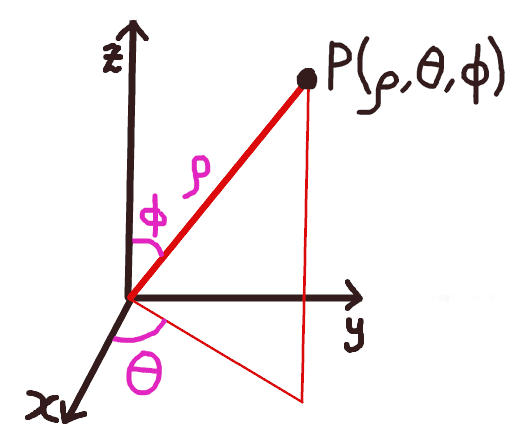
\includegraphics[scale=1.3]{sph}\centering\end{figure}
        $\rho$ (rho) is the radial distance, $\theta$ (theta) is the \textit{azimuthal angle}, and $\phi$ (phi) is the \textit{polar angle}.
\end{frame}

\begin{frame}{Integration in spherical coordinates}
    In the 2D world, we have polar coordinates, where $dA=\blue{r}\cdot dr\,d\theta$.

    \pause In 3D's spherical coordinates, we have $\boxed{\boxed{dV=\blue{\rho^2\sin\phi}\cdot d\rho\,d\theta \,d\phi}}$.

    {\scriptsize(The blue factors are Jacobians, if you want to know more about them)}

    \pause For spherical coordinates, we have:
        \[\boxed{x=\rho\sin\phi\cos\theta \qquad y=\rho\sin\phi\sin\theta \qquad z=\rho\cos\phi}\]
        \[\boxed{x^2+y^2+z^2=\rho^2}\]
    \pause\textbf{Note:} the slides use the convention of the book, where $\rho$ is the radial distance, $\theta$ is the azimuthal angle and $\phi$ is the polar angle. However, some sources swap the meanings of $\theta$ and $\phi$ and/or write $r$ instead of $\rho$, so be aware of that.
\end{frame}

\begin{frame}{Example integral in spherical coordinates (1/2)}
    \footnotesize
    \textbf{Question:} evaluate $\iiint_E xe^{x^2+y^2+z^2}\,dV$, where $E$ is the region with $x^2+y^2+z^2\leq4$ and $0\leq y\leq x$.

    \pause\textbf{Step 1:} do geometry; write $E$ in spherical coordinates:
    \[E=\left\{(\rho,\theta,\phi) \mid 0\leq\rho\leq2,~0\leq\theta\leq\frac{\pi}{4},~-\frac{\pi}{2}\leq\phi\leq\frac{\pi}{2}\right\}\]

    \pause\textbf{Step 2:} since $x=\rho\sin\phi\cos\theta$ and $x^2+y^2+z^2=\rho^2$ in spherical coordinates, we can rewrite the integrand as $\rho\sin\phi\cos\theta \,e^{\rho^2}$.

    \pause\textbf{Step 3:} set up the integral. Do not forget the Jacobian $\blue{\rho^2\sin\phi}$ for spherical coordinates!
    \[\iiint_E xe^{x^2+y^2+z^2}\,dV = \int_{-\pi/2}^{\pi/2}\int_0^{\pi/4}\int_0^2 \rho\sin\phi\cos\theta\,e^{\rho^2}\blue{\rho^2\sin\phi}\,d\rho\,d\theta\,d\phi\]
    \[=\teal{\left(\int_{-\pi/2}^{\pi/2}\sin^2\phi\,d\phi\right)}\yellow{\left(\int_0^{\pi/4}\cos\theta\,d\theta\right)}\red{\left(\int_0^2\rho^3\,e^{\rho^2}\,d\rho\right)}
 \]
    We were able to write the long integral as a product of three single-variable integrals by using the idea from slide \blue{\ref{integraltrick}}.
\end{frame}

\begin{frame}{Example integral in spherical coordinates (2/2)}
    \footnotesize
    \textbf{Step 4:} solve the integral.
    \[
        \iiint_E xe^{x^2+y^2+z^2}\,dV =\teal{\left(\int_{-\pi/2}^{\pi/2}\sin^2\phi\,d\phi\right)}\yellow{\left(\int_0^{\pi/4}\cos\theta\,d\theta\right)}\red{\left(\int_0^2\rho^3\,e^{\rho^2}\,d\rho\right)}
    \]

    \pause The red one can be solved by subbing $u=\rho^2$ (such that $du=2\rho \,d\rho$), followed by integration by parts:
    \[\red{\int_0^2\rho^3\,e^{\rho^2}\,d\rho=\frac{1}{2}\int_{0^2}^{2^2}ue^u\,du=\frac{1}{2}\left(\left[ue^u\right]_0^4-\int_0^4e^u\,du\right)=\frac{1}{2}(4e^4-(e^4-1))=\frac{3e^4+1}{2}}\]
    \pause The green one can be solved by using $\sin^2\phi=\frac{1}{2}\left(1-\cos2\phi\right)$:
    \[\teal{\int_{-\pi/2}^{\pi/2}\sin^2\phi\,d\phi=\frac{1}{2}\int_{-\pi/2}^{\pi/2}(1-\cos2\phi)\,d\phi=\frac{\pi}{2}-\frac{1}{2}\left[\frac{1}{2}\sin2\phi\right]_{-\pi/2}^{\pi/2}=\frac{\pi}{2}}\]
    \pause The orange one is relatively straightforward, so the answer is:

    \[
        \iiint_E xe^{x^2+y^2+z^2}\,dV =\teal{\left(\frac{\pi}{2}\right)}\yellow{\left(\frac{1}{2}\sqrt{2}\right)}\red{\left(\frac{3e^4+1}{2}\right)}=\boxed{\frac{\pi\sqrt2}{8}(3e^4+1)}
    \]
\scriptsize    P.S. The need to use substitution, integration by parts and a trigonometric identity makes this question harder than exam-level (no warranty). 
\end{frame}
